% Generated by paper/figures/src/fig_phase2.py 8192; do not edit by hand.
% Generated by fig_phase2.py 8192; frozen selection in gallery_8192/provenance.json.
% m4469448794852185540: Silhouettes of twelve characters are arranged in a row, each corresponding to a different backdrop of vibrant colors and cosmic themes, numbered one to twelve. Each figure wears a distinctive outfit, often featuring long coats, with various poses reflecting unique characteristics or actions. The backgrounds exhibit a mix of abstract designs, including starry skies, swirling galaxies, and fiery textures, creating a visually dynamic scene.
% m4850138611731379908: A vast desert landscape under a starry night sky, featuring rolling sand dunes illuminated by a soft glow on the horizon, with a vibrant Milky Way arching overhead.
% m5023570400257826529: A large planet with prominent rings occupies the foreground against a backdrop of deep red space, while two smaller celestial bodies are silhouetted nearby, one near the planet's rings and another near a distant sun.
% m5691444384207183173: A wooden window with blue shutters frames sheer curtains, overlooking a flower box brimming with pink and blue blossoms against a warm red wall.
\begin{figure*}[t]
\centering\sffamily\scriptsize\ifdefined\scaW\else\newlength{\scaW}\fi\setlength{\scaW}{\textwidth}
\setlength{\fboxsep}{1pt}\setlength{\lineskip}{0pt}\setlength{\lineskiplimit}{0pt}
\makebox[\textwidth][l]{\makebox[0.4975\scaW][c]{AReA}\hspace{0.0040\scaW}\makebox[0.4975\scaW][c]{\textbf{SCA (ours)}}}\\[0.0040\textwidth]
\makebox[\textwidth][l]{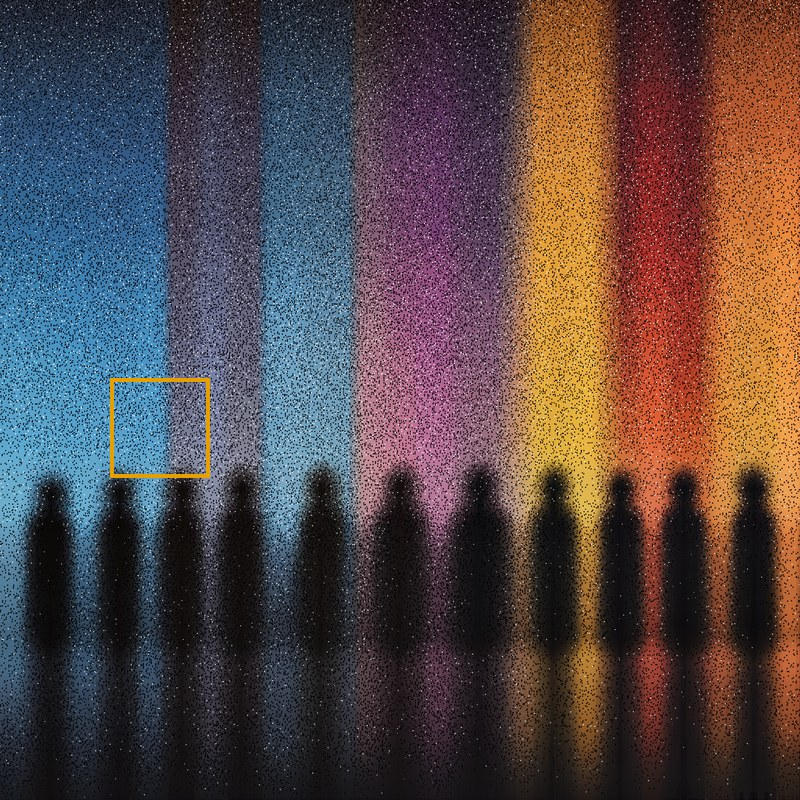
\includegraphics[height=0.2467\scaW]{figures/gallery_8192/m4469448794852185540_area.jpg}\hspace{0.0040\scaW}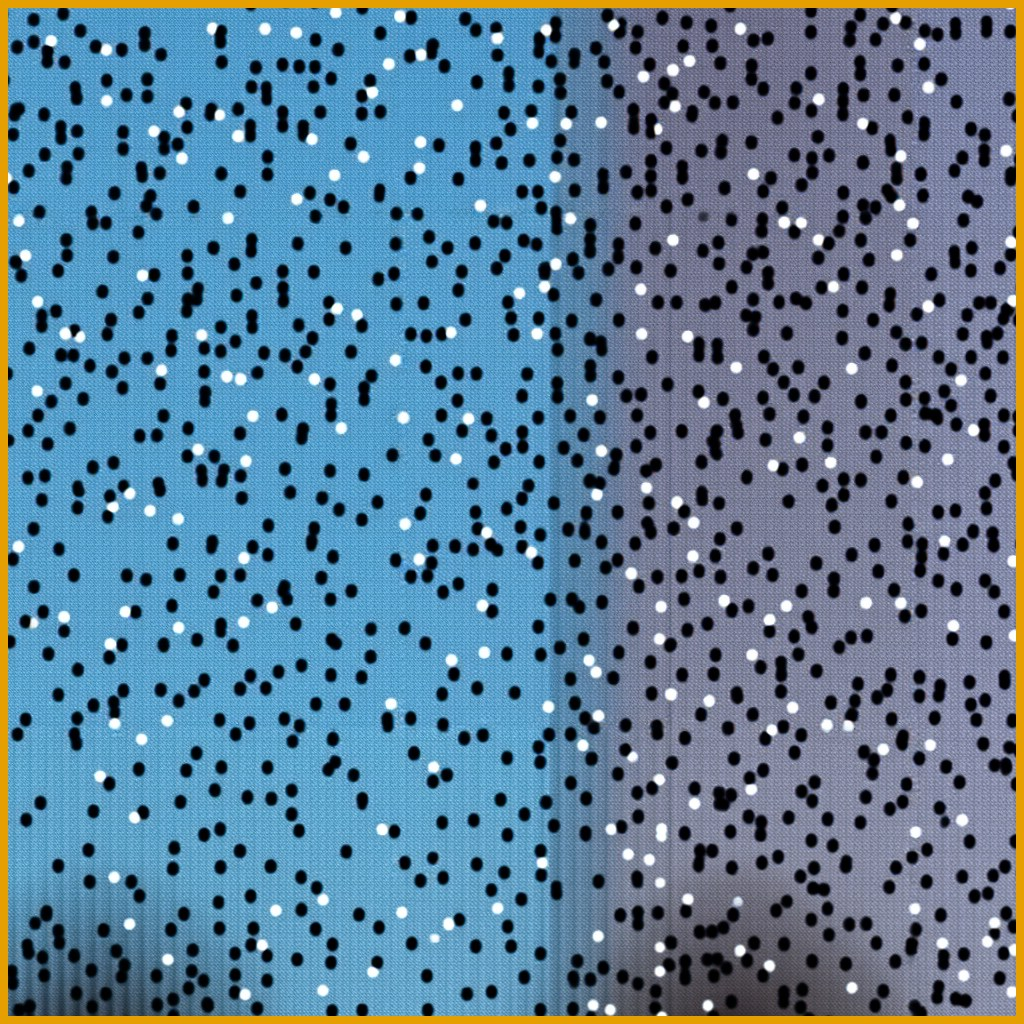
\includegraphics[height=0.2467\scaW]{figures/gallery_8192/m4469448794852185540_area_crop.jpg}\hspace{0.0040\scaW}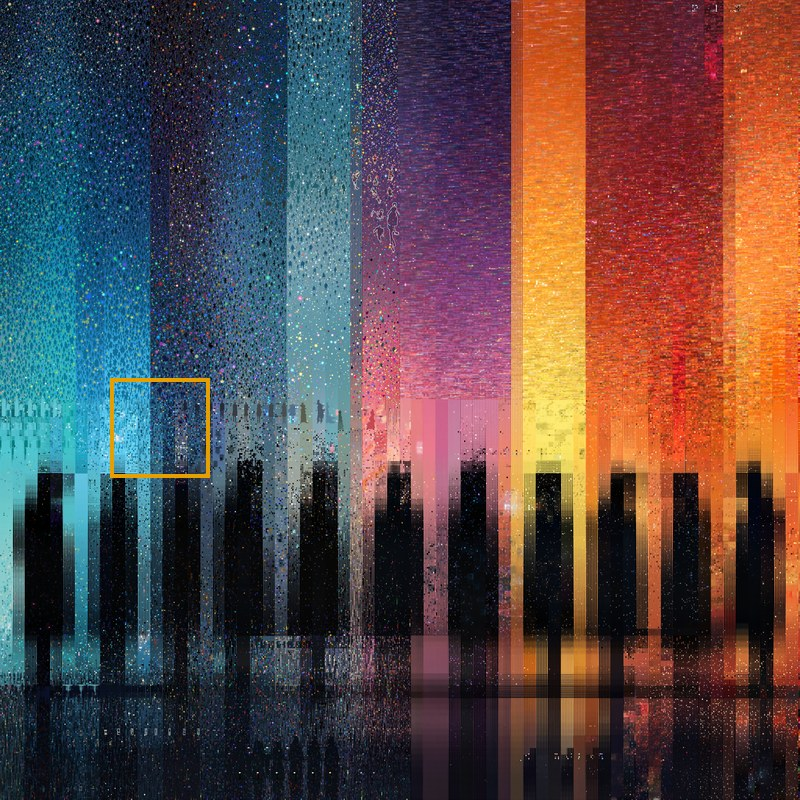
\includegraphics[height=0.2467\scaW]{figures/gallery_8192/m4469448794852185540_sca.jpg}\hspace{0.0040\scaW}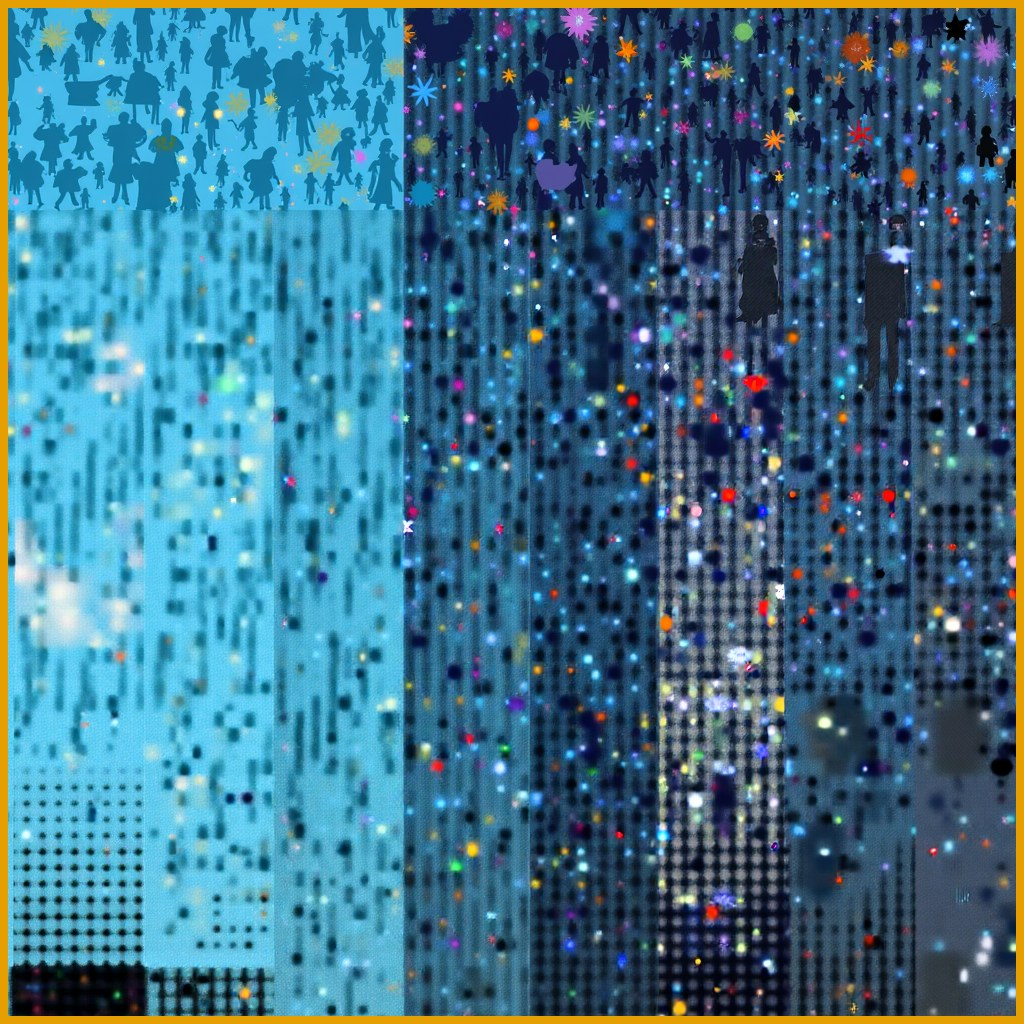
\includegraphics[height=0.2467\scaW]{figures/gallery_8192/m4469448794852185540_sca_crop.jpg}}\\[0.0040\textwidth]
\makebox[\textwidth][l]{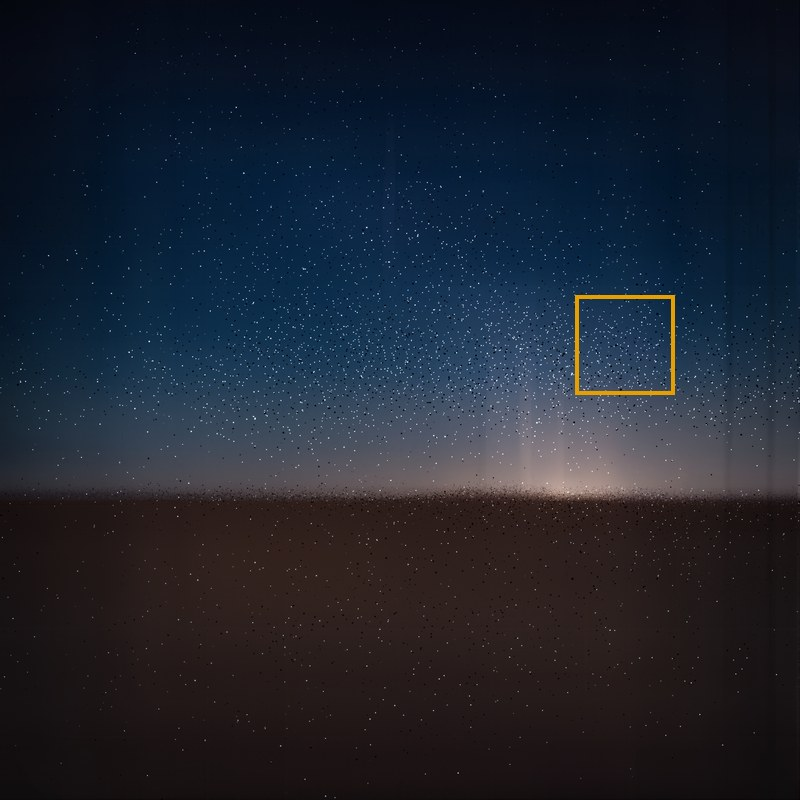
\includegraphics[height=0.2467\scaW]{figures/gallery_8192/m4850138611731379908_area.jpg}\hspace{0.0040\scaW}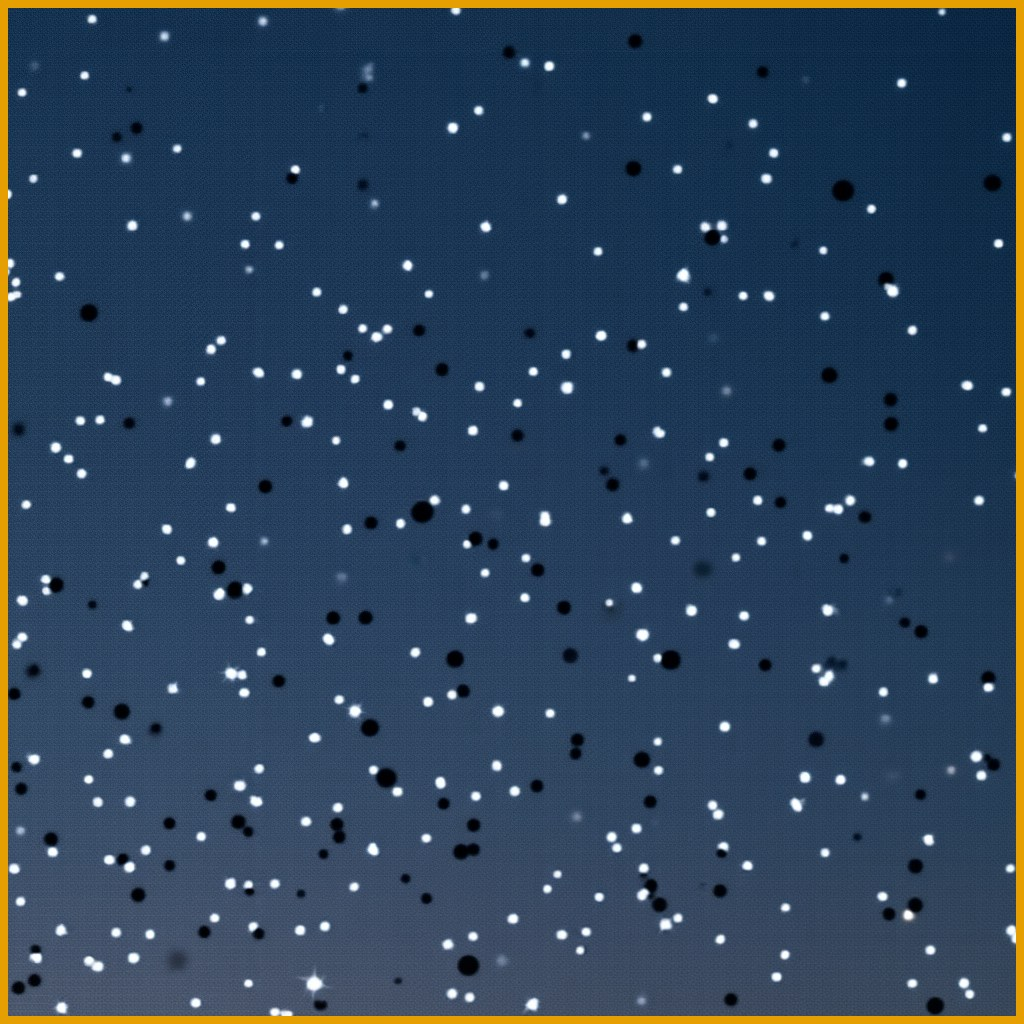
\includegraphics[height=0.2467\scaW]{figures/gallery_8192/m4850138611731379908_area_crop.jpg}\hspace{0.0040\scaW}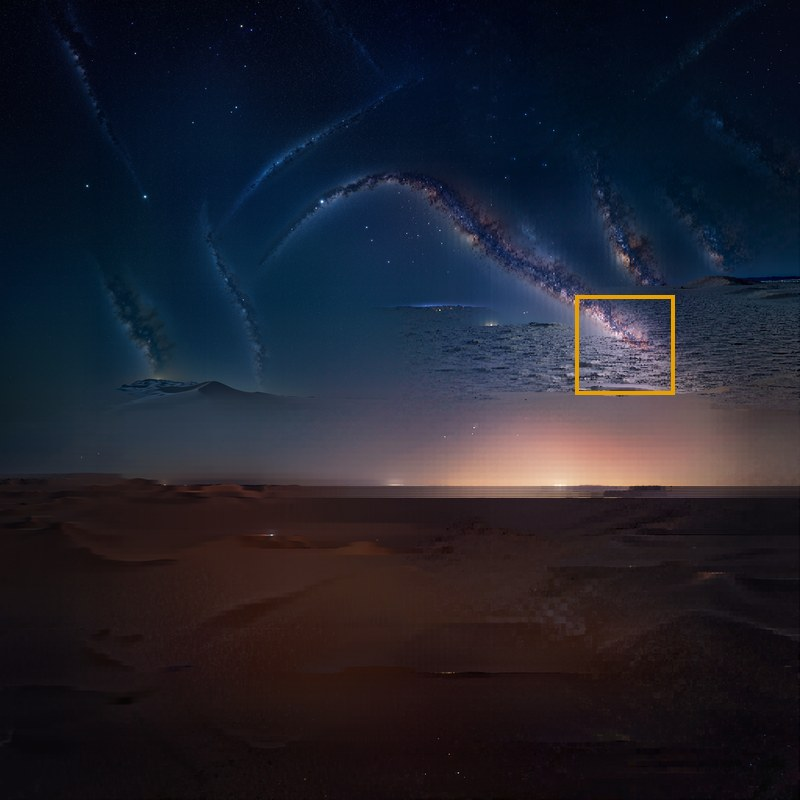
\includegraphics[height=0.2467\scaW]{figures/gallery_8192/m4850138611731379908_sca.jpg}\hspace{0.0040\scaW}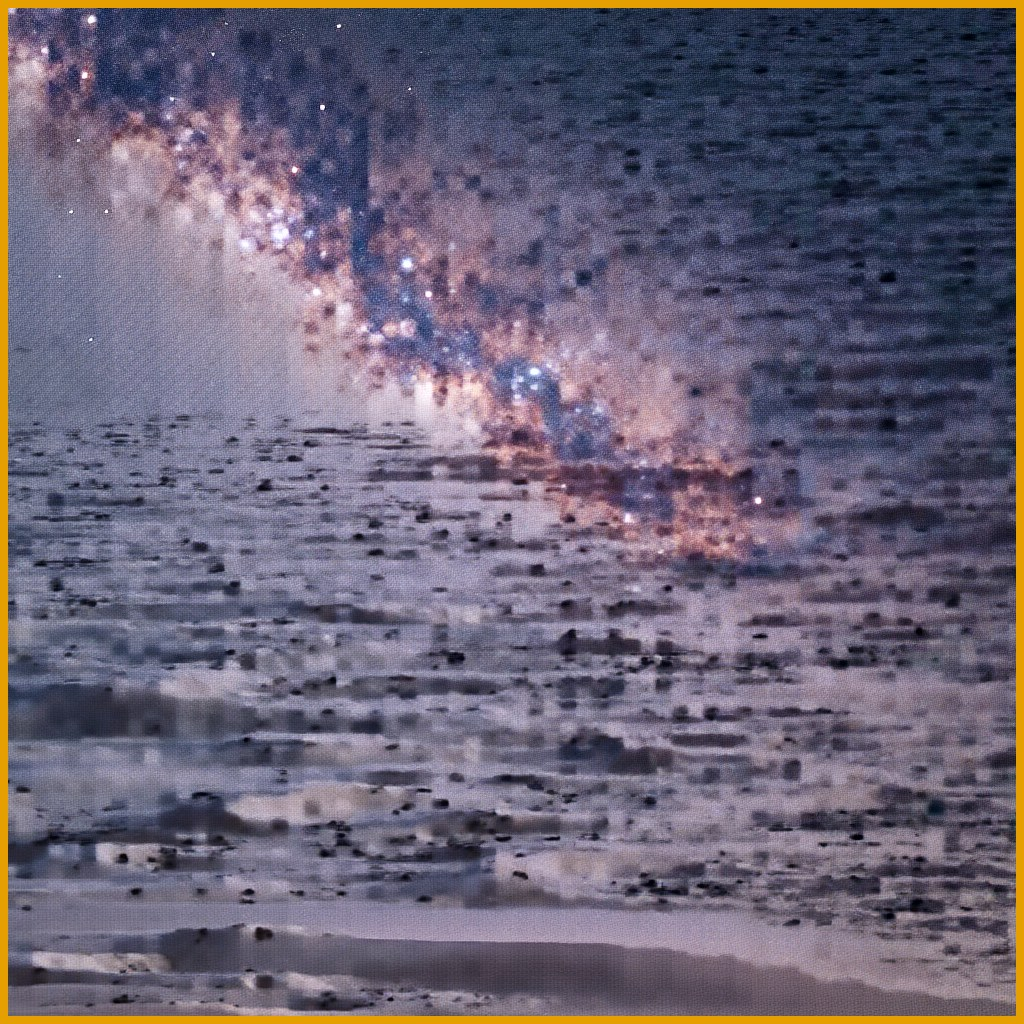
\includegraphics[height=0.2467\scaW]{figures/gallery_8192/m4850138611731379908_sca_crop.jpg}}\\[0.0040\textwidth]
\makebox[\textwidth][l]{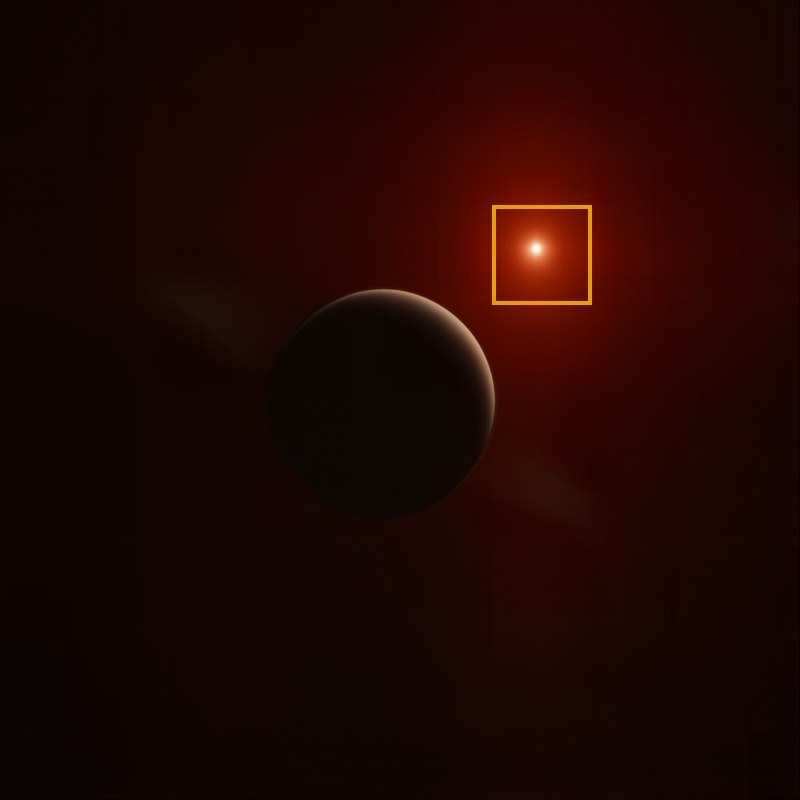
\includegraphics[height=0.2467\scaW]{figures/gallery_8192/m5023570400257826529_area.jpg}\hspace{0.0040\scaW}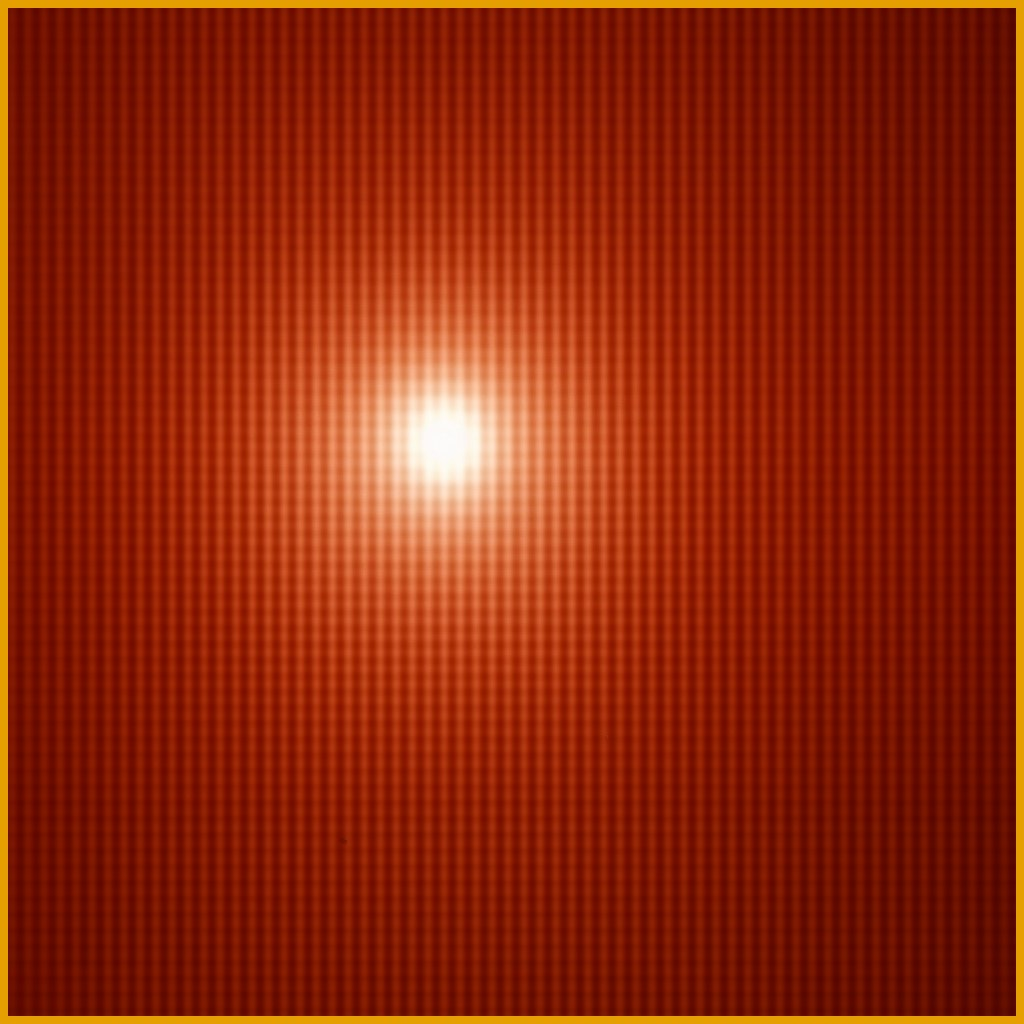
\includegraphics[height=0.2467\scaW]{figures/gallery_8192/m5023570400257826529_area_crop.jpg}\hspace{0.0040\scaW}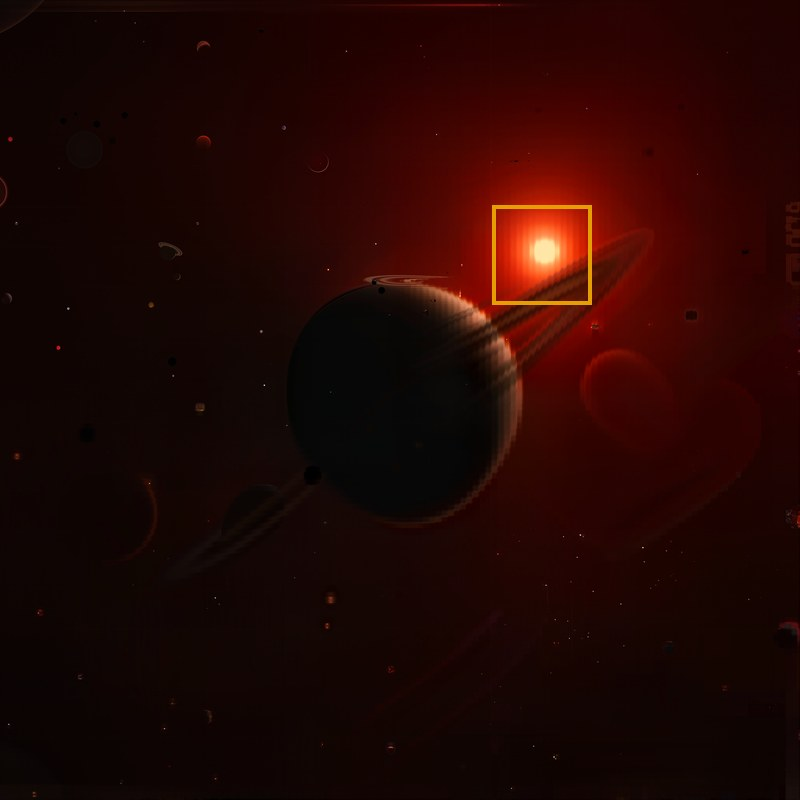
\includegraphics[height=0.2467\scaW]{figures/gallery_8192/m5023570400257826529_sca.jpg}\hspace{0.0040\scaW}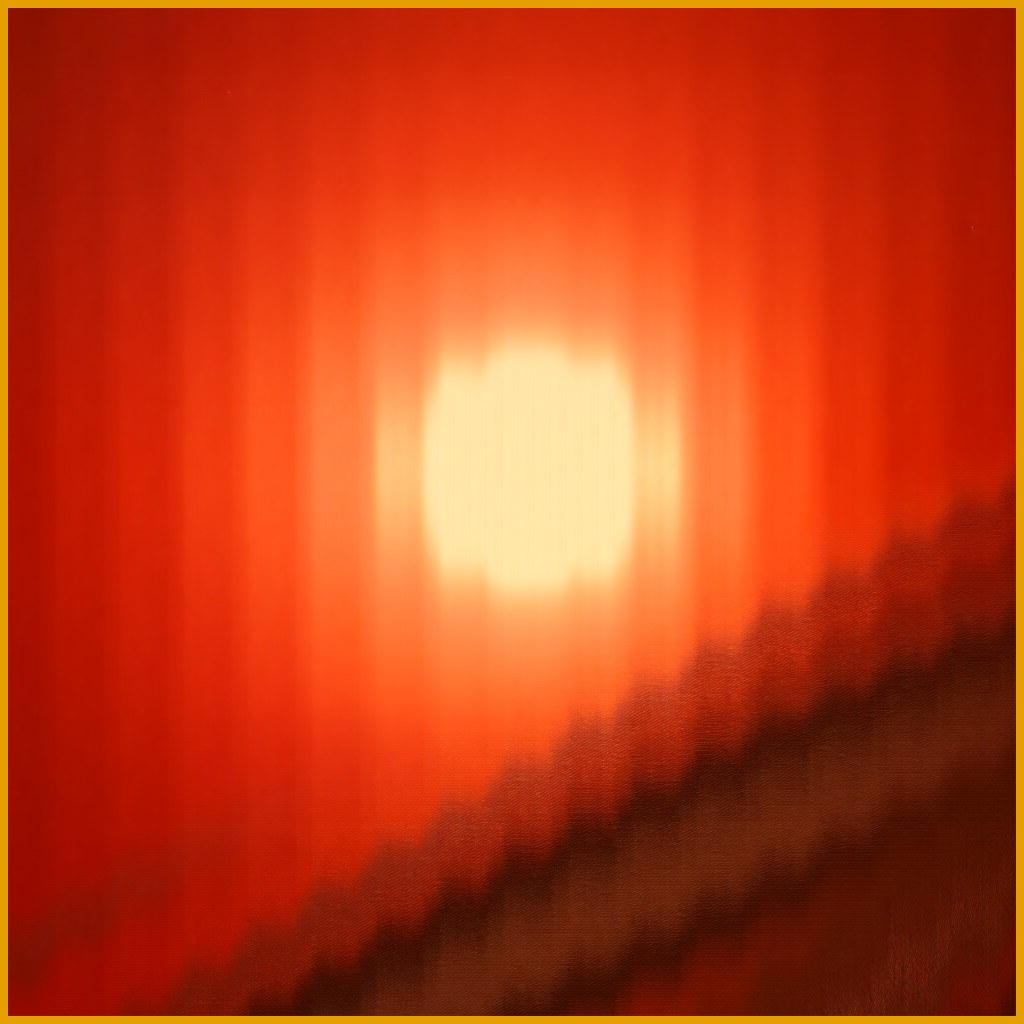
\includegraphics[height=0.2467\scaW]{figures/gallery_8192/m5023570400257826529_sca_crop.jpg}}\\[0.0040\textwidth]
\makebox[\textwidth][l]{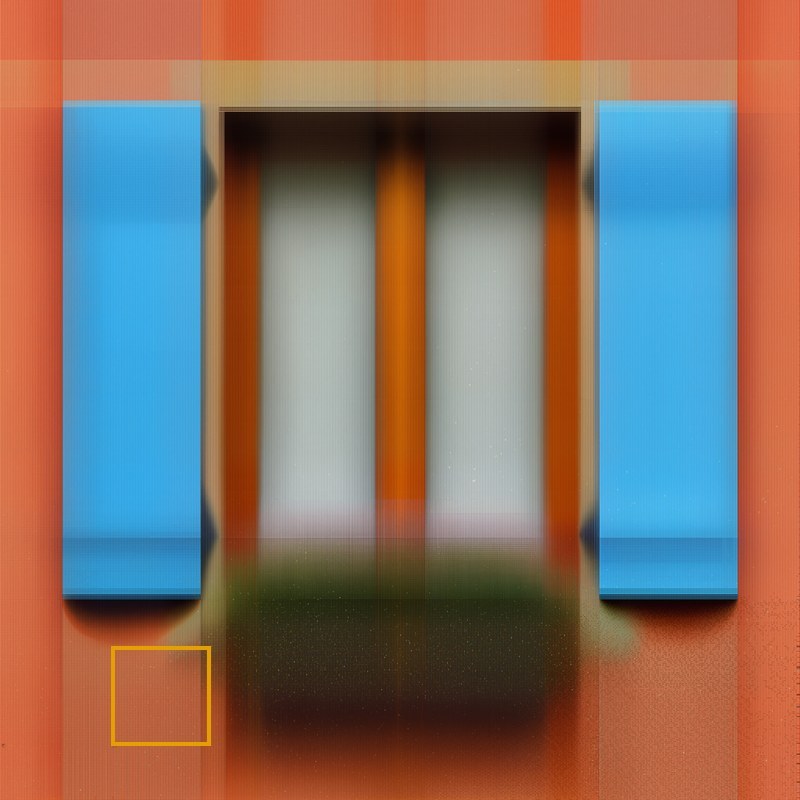
\includegraphics[height=0.2467\scaW]{figures/gallery_8192/m5691444384207183173_area.jpg}\hspace{0.0040\scaW}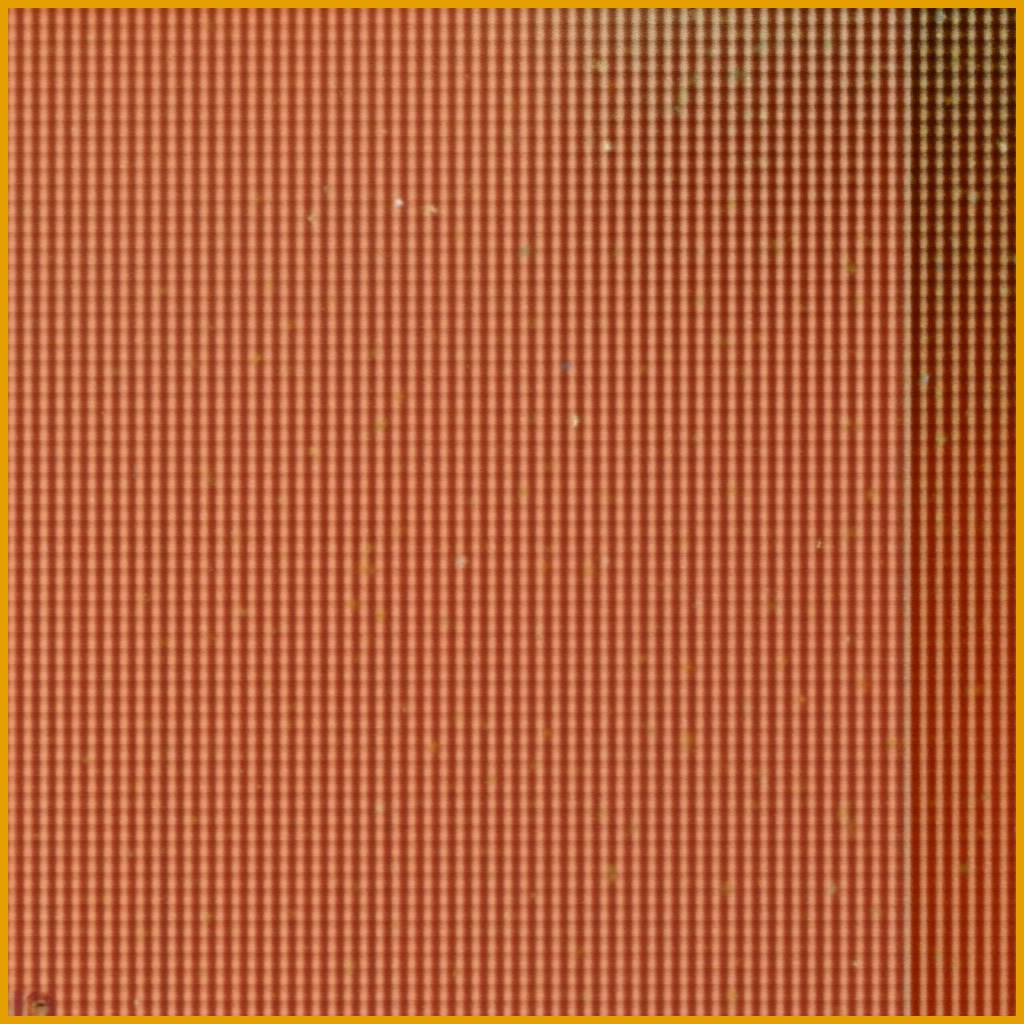
\includegraphics[height=0.2467\scaW]{figures/gallery_8192/m5691444384207183173_area_crop.jpg}\hspace{0.0040\scaW}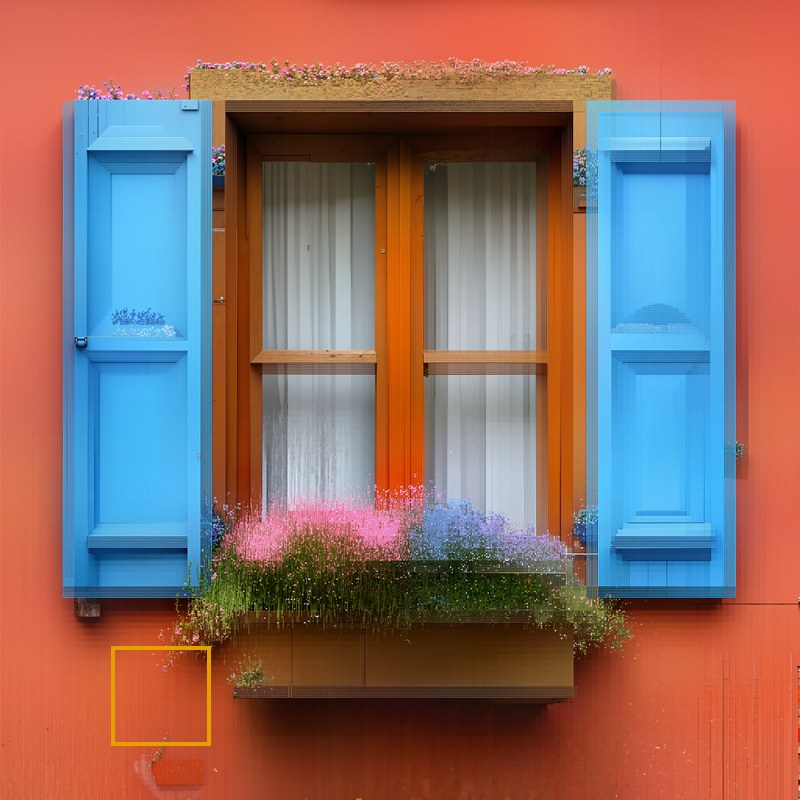
\includegraphics[height=0.2467\scaW]{figures/gallery_8192/m5691444384207183173_sca.jpg}\hspace{0.0040\scaW}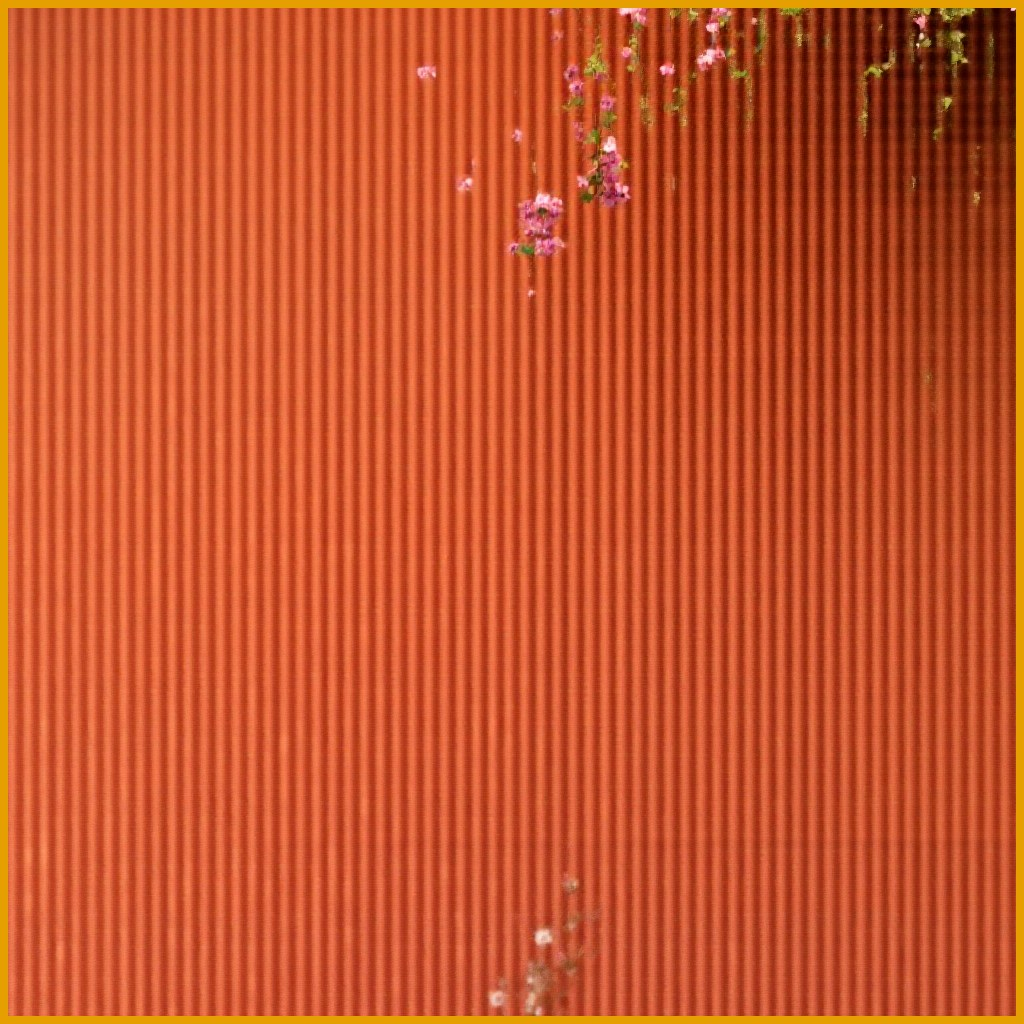
\includegraphics[height=0.2467\scaW]{figures/gallery_8192/m5691444384207183173_sca_crop.jpg}}
\rmfamily\normalsize
\caption{\textbf{Partial qualitative results at $8192^2$.} 4 prompts sampled uniformly from the 11 non-development prompts with completed AReA and SCA outputs at the figure snapshot; this is not the final evaluation set. Each full image is followed by its native-pixel crop. FLUX.1-dev, seed 0, 28 steps, guidance 4.5. The subset was not selected by image quality; completion order may differ from the full benchmark. Visible grid and stripe artifacts remain in both methods at this scale. Crop locations maximize edge energy averaged across the methods shown. Prompt selection uses seed 17; source hashes and crop coordinates are archived with the figure.}
\label{fig:gallery_8192}
\end{figure*}
